\chapter{Numerical results}
We have implemented the Finite Volume Method for solving the shallow water equations in 1D and tested it on two different dam break problems
\footnote{Code and small animations can be found at github, visit \url{https://github.com/MelissaJessen/Shallow-Water-Equations}.}.

\section{Metod of manufactured solutions}
Method of manufactured solutions (MMS) was used to verify the implementation.
We use a manufactured solution for $h(x,t)$ and $u(x,t)$.
Choose a simple sine wave function for the water height $h$ and a corresponding $u$ that satisfies the shallow water equations.
Consider
\begin{align*}
    h(x,t) &= h_0 + A \cos(\omega t - kx), \\
    u(x,t) &= \frac{ A \omega }{k h_0}  \cos(\omega t - kx),
\end{align*} 
where $h_0$ is the constant base depth, $A$ is the amplitude of the wave, $k$ is the wave number, and $\omega$ is the angular frequency.

We begin by computing the source terms $S_h$ and $S_u$.
First we compute the partial derivatives
\begin{align*}
    h_t &= ,\\
    u_t &=  \\
\end{align*}
which gives (using the chain rule)
\begin{align*}
    {(hu)}_x &= h_x u + h u_x \\
    &= 
\end{align*}

\section{The 1D Dam Break Problem}
The numerical solution to the 1D Dam Break Problem using the FVM, together with the true solution can be seen in \autoref{fig:1D_dam_break}.

\begin{figure}[H]
    \centering
    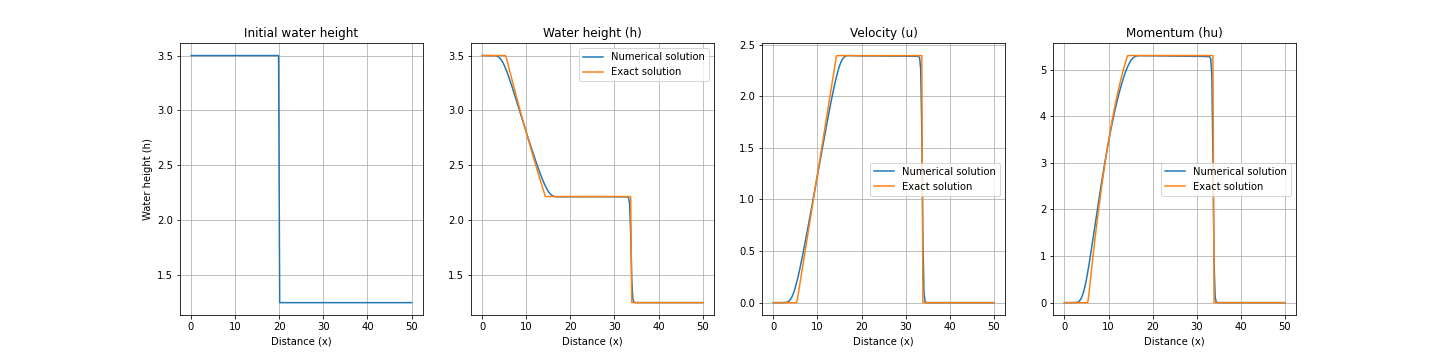
\includegraphics[width=0.6\textwidth]{plots/sol_1D_val.png}
    \caption{1D dam break problem.}\label{fig:1D_dam_break}
\end{figure}


\section{2D idealised Circular Dam Break Problem}
Consider the idealised circular dam break problem with a horizontal bottom.
We assume there is an infinitely thin circular wall at radius $R = 2.5 m$ is a square domain of size $40 m \times 40 m$ with centre at $(x_c,y_c) = (20 m, 20 m)$.
The initial conditions are
\begin{align*}
    h(x,y,0) &= \begin{cases}
        2.5 \text{ }m, & \text{if } \sqrt{ {(x-x_c)}^2 + {(y-y_c)}^2 } \leq R, \\
        0.5 \text{ }m, & \text{otherwise},
    \end{cases} \\
    u(x,y,0) &= 0, \\
    v(x,y,0) &= 0.
\end{align*}
Use the WAF method (chapter 11) along with a second-order dimensional splitting scheme (chapter 12).
CFL-condition: $C_{cfl} = 0.9$.
van Leer limiter. Mesh: $200 \times 200$.

Solve the 1D inhomoegeneous system and compare.


\section{Test cases}

Test case 1:

\begin{figure}[H]
    \centering
    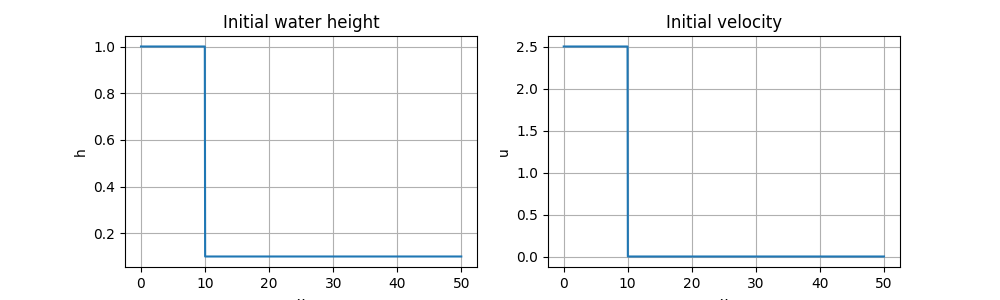
\includegraphics[width=0.5\textwidth]{C:/Users/Matteo/Shallow-Water-Equations/plots/toro_test1_initial.png}
    \caption{Initial conditions for the test case.}\label{fig:toro_test1_initial}
\end{figure}


\begin{figure}[H]
    \centering
    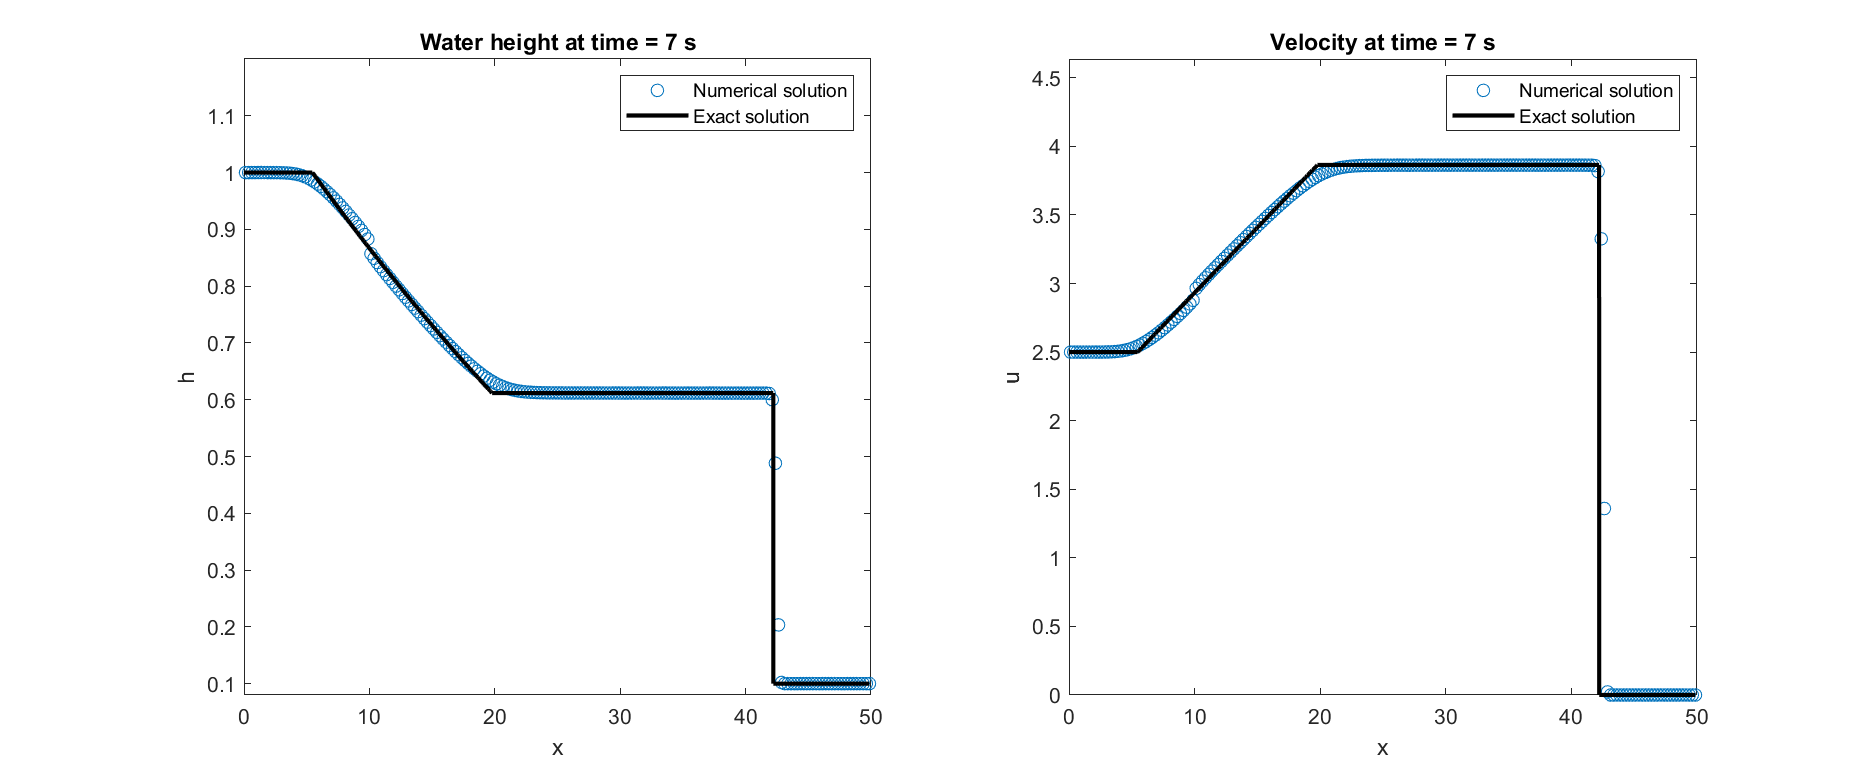
\includegraphics[width=0.5\textwidth]{C:/Users/Matteo/Shallow-Water-Equations/plots/toro_test1_final.png}
    \caption{Final solution for the test case.}\label{fig:toro_test1_final}
\end{figure}


Test case 2: 


\begin{figure}[H]
    \centering
    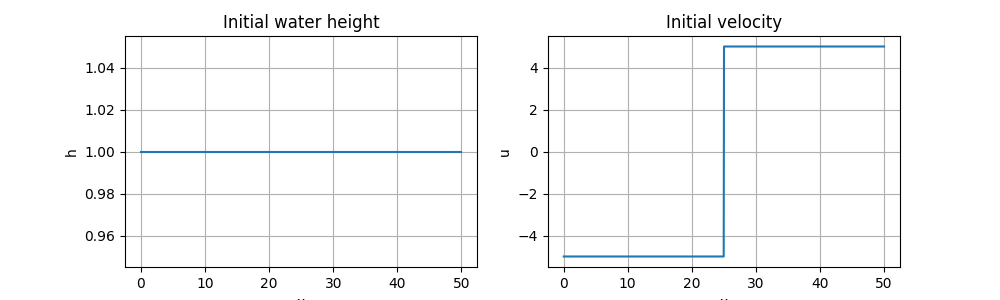
\includegraphics[width=0.5\textwidth]{C:/Users/Matteo/Shallow-Water-Equations/plots/toro_test2_initial.png}
    \caption{Initial conditions for the test case.}\label{fig:toro_test2_initial}
\end{figure}

\begin{figure}[H]
    \centering
    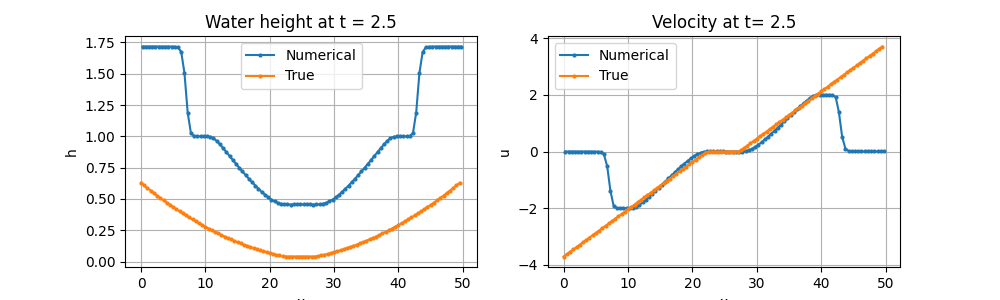
\includegraphics[width=0.5\textwidth]{C:/Users/Matteo/Shallow-Water-Equations/plots/toro_test2_final.png}
    \caption{Final solution for the test case.}\label{fig:toro_test2_final}
\end{figure}


Test case 3:

\begin{figure}[H]
    \centering
    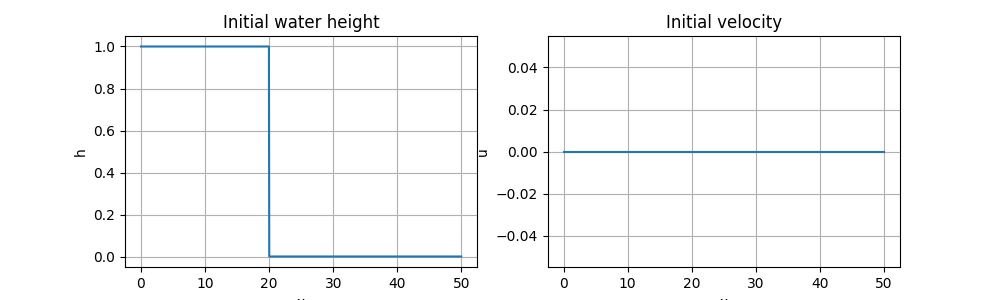
\includegraphics[width=0.5\textwidth]{C:/Users/Matteo/Shallow-Water-Equations/plots/toro_test3_initial.png}
    \caption{Initial conditions for the test case.}\label{fig:toro_test3_initial}
\end{figure}

\begin{figure}[H]
    \centering
    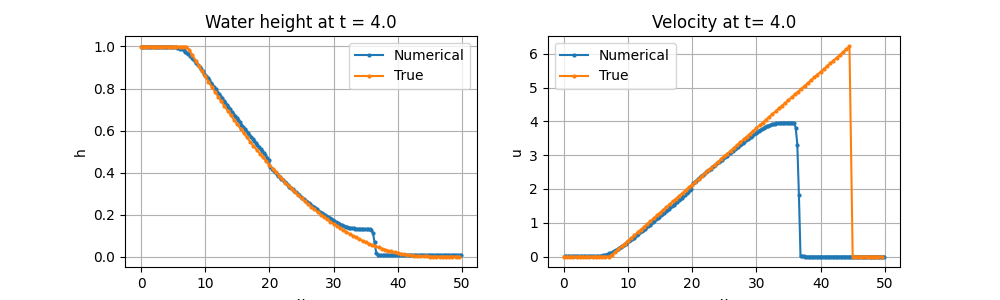
\includegraphics[width=0.5\textwidth]{C:/Users/Matteo/Shallow-Water-Equations/plots/toro_test3_final.png}
    \caption{Final solution for the test case.}\label{fig:toro_test3_final}
\end{figure}


Test case 4:

\begin{figure}[H]
    \centering
    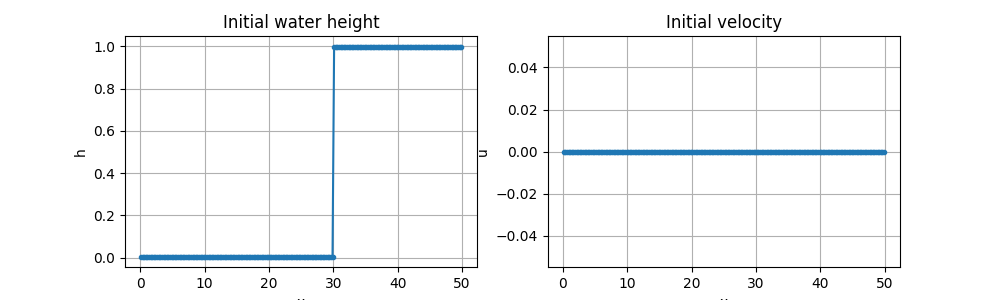
\includegraphics[width=0.5\textwidth]{C:/Users/Matteo/Shallow-Water-Equations/plots/toro_test4_initial.png}
    \caption{Initial conditions for the test case.}\label{fig:toro_test4_initial}
\end{figure}

\begin{figure}[H]
    \centering
    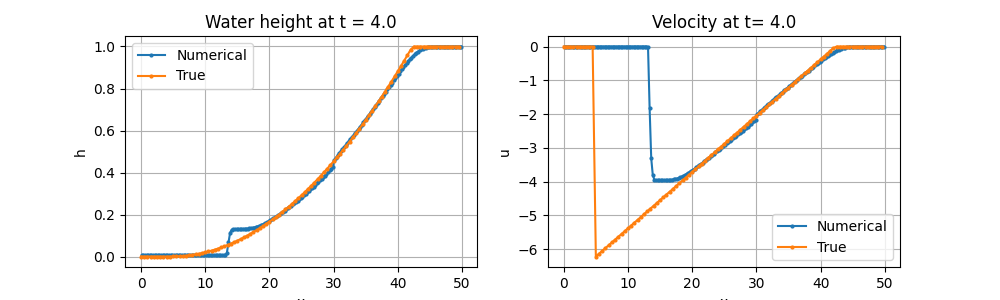
\includegraphics[width=0.5\textwidth]{C:/Users/Matteo/Shallow-Water-Equations/plots/toro_test4_final.png}
    \caption{Final solution for the test case.}\label{fig:toro_test4_final}
\end{figure}



Test case 5:

\begin{figure}[H]
    \centering
    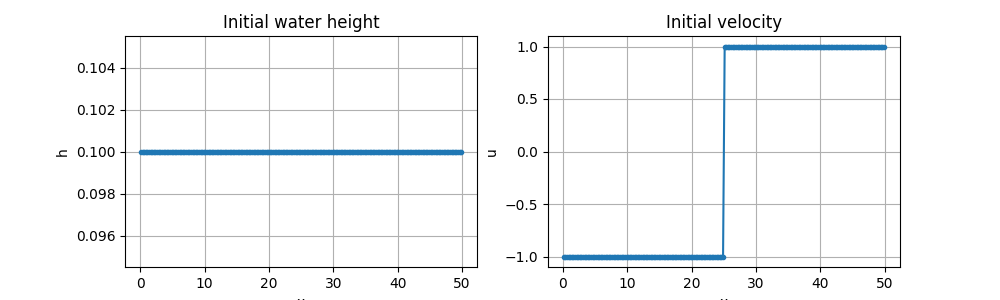
\includegraphics[width=0.5\textwidth]{C:/Users/Matteo/Shallow-Water-Equations/plots/toro_test5_initial.png}
    \caption{Initial conditions for the test case.}\label{fig:toro_test5_initial}
\end{figure}

\begin{figure}[H]
    \centering
    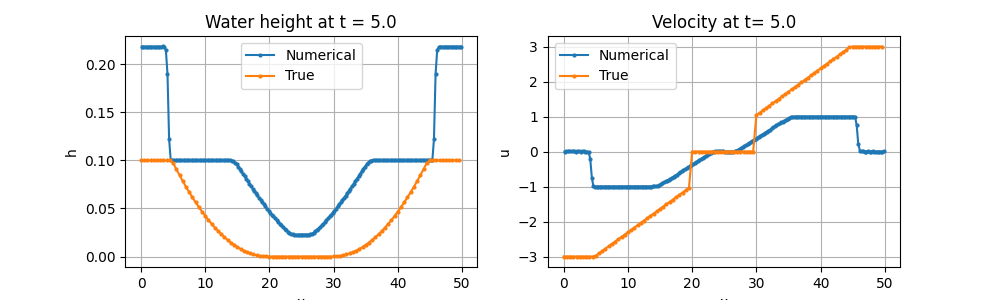
\includegraphics[width=0.5\textwidth]{C:/Users/Matteo/Shallow-Water-Equations/plots/toro_test5_final.png}
    \caption{Final solution for the test case.}\label{fig:toro_test5_final}
\end{figure}


